%
% fig-methode.tex
%
% (c) 2026 Prof Dr Andreas Müller
%
\begin{figure}
\centering
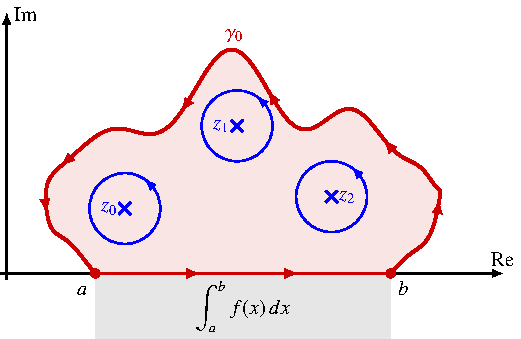
\includegraphics{chapters/030-integration/images/methode.pdf}
\caption{Die komplexe Wegintegration ermöglicht das Integral der
reellen Funktion $f(x)$ durch ein Integral einer geeigneten
komplexen Funktion $f(z)$ entlang des Weges
$\gamma_0$ und auszudrücken.
Falls im Inneren des roten Gebietes Singularitäten der Funktion $f(z)$
auftreten, symbolisiert durch die blauen Punkte, dann kommen 
noch Kurvenintegrale entlang kleinen Kreisen um die Singularitäten
hinzu.
\label{buch:integration:residuen:fig:methode}}
\end{figure}
